\documentclass[11pt]{article}
\usepackage{tikz}

\usetikzlibrary{arrows}

\title{Bless, a pager\footnote{not like less}}
\author{void-}

\begin{document}
\maketitle
\section*{Overview}
\subsection*{Goal}
The Sender wishes to send a message to (i.e. page) the Receiver in real time.
The location of the Receiver should be private and the confidentiality,
integrity, and authenticity of the message should be preserved. The Sender must
also be approved to send messages to the Receiver, that is to say, not just
anyone can send a message to the Receiver. The system should work even if the
Receiver is behind a NAT.

\section*{An illustration}
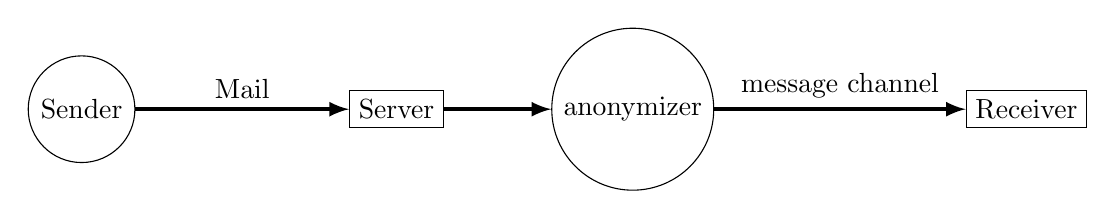
\begin{tikzpicture}
\node[draw, circle] at (0,0) (sender) {Sender};
\node[draw, rectangle] at (4,0) (server) {Server};
\node[draw, circle] at (7,0) (anonymizer) {anonymizer};
\node[draw, rectangle] at (12,0) (receiver) {Receiver};

\draw[arrows={-latex}, line width=.5mm]
  (sender) to node[above] {Mail} (server);
\draw[arrows={-latex}, line width=.5mm] (server) to (anonymizer);
\draw[arrows={-latex}, line width=.5mm]
  (anonymizer) to node[above] {message channel} (receiver);
\end{tikzpicture}

\section*{How it works}
Alice is the Sender, Bob the Receiver. Alice wants to send a message to Bob
while Bob is in an undisclosed location with internet access. Prior to this,
Alice and Bob exchanged public keys and the routing address of Bob's server(the
Server).

Bob, somewhere in the world, is connected to a NATed wifi with his device.
Using an anonymity network, Bob initially makes a TCP connection to the Server.
This bootstraps the message channel. Bob will then send a UDP packet to the
Server; this creates a UDP hole punch in the NAT to facilitate a push protocol
between the Server and Bob. The Server will send periodic, empty UDP
packets\footnote{it doesn't matter if these are authenticated, an attacker can
keep the connection alive}
over the message channel to keep the hole punch active.

If Alice sends the Server a message, the Server will authenticate it and
forward this onto Bob. If Bob changes his physical location in the world, the
UDP packets sent by the Server will unknowingly go undelivered.

\subsection*{Why isn't Bob just a Tor hidden service that moves?}
\begin{itemize}
\item Bob's mobile device has a small battery so a push protocol is desired
\item The use of an anonymizer between connections to the server is optional
\item Alice is considered an luser\footnote{local user}, she is neither capable
of connecting to the Tor network nor capable of running sophisticated software.
% Consider Alice being able to run `statically-linked' python scripts;
%  A mail server is hard to set up and requires root permissions
% She's still unable to make a TLS connection, this is too much
\item This should be a real time protocol. Reducing latency is desired and the
anonymizer in the message channel is optional.
\item I wanted to design my own protocol.
\end{itemize}

\pagebreak
\section*{Definitions}
\begin{itemize}
\item Sender \\
The entity that wishes to send a single message to the Receiver via the Server.
This can represent a number of authenticated individuals.
\item Server \\
The publicly routable server that authenticates messages from the Sender and
forwards them to the Receiver. Generally, the Server and the Receiver are
owned by the same individual.
\item Receiver \\
The entity that should receive a message from the Sender via the Server. The
Receiver's physical location in the world is consider private.
\item Message channel \\
The private communication channel established between the Server and Receiver.
\item Stale \\
When the message channel is stale, it means the Receiver has moved unbeknownst
to the Server. The Server will continue to attempt to communicate with the
Receiver using this channel even though the Receiver isn't listening.
\end{itemize}
\pagebreak

\section*{Message format}
%Can this use some form of OTR or a ratchet?
\subsection*{Sender $\rightarrow$ Server}
\begin{tabular}{c c c}
  $Sig_{k_{sender}}\left(mail\right)$ & $256$B &
    Signature of the entire rest of the mail contents\\
  $E_{k_{server}}\left(k_{sym}\right)$ & $256$B &
    Encryption of a symmetric key under the Server's public key\\
  $E_{k_{sym}}\left(m\right)$ & $\left[0, 2^{16} - 512 \right]$B &
    Encryption of the message with the symmetric key
\end{tabular}
The current design uses deterministic encryption. It will not prevent replay
attacks.

\subsection*{Server $\rightarrow$ Receiver}

\subsection*{Steps from Server $\rightarrow$ Receiver}
\begin{itemize}
  \item Receiver establishes TCP connection to Server
  \item Diffie-Hellman key exchange between Server and Receiver yields
  $k_{mac}$ and $k_{enc}$
  \item Close TCP connection and create UDP hole punch
  %use OTR here by tricks with the mac key
  \item Receiver receives, over UDP, $E_{k_{mac}}\left{\right}$

\end{itemize}

\end{document}
